%%
%% This is file `thesis.tex',
%% generated with the docstrip utility.
%%
%% The original source files were:
%%
%% nudtpaper.dtx  (with options: `thesis')
%% 
%% This is a generated file.
%% 
%% Copyright (C) 2012 by Liu Benyuan <liubenyuan@gmail.com>
%% 
%% This file may be distributed and/or modified under the
%% conditions of the LaTeX Project Public License, either version 1.3a
%% of this license or (at your option) any later version.
%% The latest version of this license is in:
%% 
%% http://www.latex-project.org/lppl.txt
%% 
%% and version 1.3a or later is part of all distributions of LaTeX
%% version 2004/10/01 or later.
%% 
%% To produce the documentation run the original source files ending with `.dtx'
%% through LaTeX.
%% 
%% Any Suggestions : LiuBenYuan <liubenyuan@gmail.com>
%% Thanks Xue Ruini <xueruini@gmail.com> for the thuthesis class!
%% Thanks sofoot for the original NUDT paper class!
%% 
%1. 规范硕士导言
% \documentclass[master,ttf]{nudtpaper}
%2. 规范博士导言
% \documentclass[doctor,twoside,ttf]{nudtpaper}
%3. 如果使用是Vista
% \documentclass[master,ttf,vista]{nudtpaper}
%4. 建议使用OTF字体获得较好的页面显示效果
%   OTF字体从网上获得,各个系统名称统一,不用加vista选项
%   如果你下载的是最新的(1201)OTF英文字体,建议修改nudtpaper.cls,使用
%   Times New Roman PS Std
% \documentclass[doctor,twoside,otf]{nudtpaper}
%5. 如果想生成盲评,传递anon即可,仍需修改个人成果部分
% \documentclass[master,otf,anon]{nudtpaper}
%
\documentclass[master,otf]{nudtpaper}
\usepackage{mynudt}

\classification{TP957}
\serialno{0123456}
\confidentiality{公开}
\UDC{}
\title{国防科大学位论文\LaTeX{}模板\\
使用手册}
\displaytitle{国防科学技术大学学位论文\LaTeX{}模板}
\author{张三}
\zhdate{\zhtoday}
\entitle{How to Use the \LaTeX{} Document Class for NUDT Dissertations}
\enauthor{Zhang San}
\endate{\entoday}
\subject{通信与信息工程}
\ensubject{Information and Communication Engineering}
\researchfield{自动目标识别与模糊工程}
\supervisor{李四\quad{}教授}
\cosupervisor{王五\quad{}副教授} % 没有就空着
\ensupervisor{Professor Li Si}
\encosupervisor{}
\papertype{工学}
\enpapertype{Engineering}
% 加入makenomenclature命令可用nomencl制作符号列表。

\begin{document}
\graphicspath{{figures/}}
% 制作封面,生成目录,插入摘要,插入符号列表 \\
% 默认符号列表使用denotation.tex,如果要使用nomencl \\
% 需要注释掉denotation,并取消下面两个命令的注释。 \\
% cleardoublepage% \\
% printnomenclature% \\
\maketitle
\frontmatter
\tableofcontents
\listoftables
\listoffigures

\midmatter
\begin{cabstract}
国防科学技术大学是一所直属中央军委的综合性大学。1984年,学校经国务院、中央军委和教育部批准首批成立研究生院,%
肩负着为全军培养高级科学和工程技术人才与指挥人才,培训高级领导干部,从事先进武器装备和国防关键技术研究的重要任务。%
国防科技大学是全国重点大学,也是全国首批进入国家“211工程” 建设并获中央专项经费支持的全国重点院校之一。%
学校前身是1953年创建于哈尔滨的中国人民解放军军事工程学院,简称“哈军工”。
\end{cabstract}
\ckeywords{国防科学技术大学; 211; 哈军工}

\begin{eabstract}
National University of Defense Technology is a comprehensive national key university based in Changsha, %
Hunan Province, China. It is under the dual supervision of the Ministry of National Defense %
and the Ministry of Education, designated for Project 211 and Project 985, %
the two national plans for facilitating the development of Chinese higher education. %

NUDT was originally founded in 1953 as the Military Academy of Engineering in Harbin of Heilongjiang Province. %
In 1970 the Academy of Engineering moved southwards to Changsha and was renamed Changsha Institute of Technology.%
 The Institute changed its name to National University of Defense Technology in 1978.

\end{eabstract}
\ekeywords{NUDT; MND; ME}


\begin{denotation}

\item[HPC] 高性能计算 (High Performance Computing)
\item[cluster] 集群
\item[Itanium] 安腾
\item[SMP] 对称多处理
\item[API] 应用程序编程接口
\item[PI]	聚酰亚胺
\item[MPI]	聚酰亚胺模型化合物,N-苯基邻苯酰亚胺
\item[PBI]	聚苯并咪唑
\item[MPBI]	聚苯并咪唑模型化合物,N-苯基苯并咪唑
\item[PY]	聚吡咙
\item[PMDA-BDA]	均苯四酸二酐与联苯四胺合成的聚吡咙薄膜
\item[$\Delta G$]  	活化自由能~(Activation Free Energy)
\item [$\chi$] 传输系数~(Transmission Coefficient)
\item[$E$] 能量
\item[$m$] 质量
\item[$c$] 光速
\item[$P$] 概率
\item[$T$] 时间
\item[$v$] 速度

\end{denotation}


%书写正文,可以根据需要增添章节; 正文还包括致谢,参考文献与成果
\mainmatter
\chapter{绪论}

\section{课题研究背景}

\subsection{计算机硬件系统的并行化与异构化趋势}
计算机行业从它诞生伊始就保持着日新月异的发展势头。摩尔定律(Moore's Law)FIXME:citehere的神奇预言
在过去的半个世纪中准确地反映了半导体与集成电路工业的发展速度:
集成电路上的晶体管数量每18个月翻一番。在摩尔定律的作用下,单个微处理器(microprocessor)的时钟频率
越来越高,处理器性能也随之不断提高。早期计算机均采用单一微处理器作为计算部件,其性能的提高主要依赖
微处理器运算速度的提高。但随着计算机行业持续快速的发展,仅仅提高单个处理器的运算速度已经不足以使
整个计算机系同的性能得到明显提升。

首先,单个处理器的性能提高有其极限,由于功耗问题FIXME:citehere以及晶体管器件本身物理特性的限制,
单个微处理器的频率不可能无限提高;其次,随着计算机系统结构日益复杂和多样化,
访存延迟、存储器带宽等因素可能成为制约性能的主要瓶颈;此外,程序中可发掘的指令级
并行(ILP)能力有限,单一指令流已经难以充分利用高速处理器的处理能力。
因此,当今业界主流厂商已经将眼光投向并行硬件,包括多处理器(multi-processor)计算机、
多核处理器(multi-core processor)以及面向特定应用的协处理器(coprocessor),
希望通过为用户提供多个处理器或为特定应用需求提供专用处理器来获得更高的性能。

2001年IBM推出了首款通用双核(dual-core)处理器,此后,各大主流厂商相继推了不同系列的多核处理器,单个
处理器包括的核心数目不等,有的处理器核心数目可以达到16或者更多(如AMD Opteron系列,Intel Xeon系列等)。
短短几年之内,多核处理器已经占据市场主流位置,从超级计算机到高性能服务器,从桌面PC到移动通信设备,
多核处理器在许多领域都得到了广泛应用。

协处理器一般是针对特定应用而设计的处理器,如浮点计算、图形处理、信号处理、加密解密等。相较于通用
处理器,协处理器可能缺乏某些功能,但在特定的功能上具备突出的性能优势。许多计算机系统都配备一个或
多个协处理器,用以辅助CPU执行计算。图形处理器(Graphics Processor Unit, GPU)是当前应用最为广泛的一类协处理器,
它最开始被专门设计于图形处理问题,协助CPU完成图形渲染等工作,但近几年GPU已经越来越成为一种“通用”计算设备,
主流GPU厂商已经为在GPU上执行通用计算提供支持软硬件支持采取了许多努力。
GPU采用流处理(stream processing)编程模型,这是一种类似于SIMD(Single Instruction Multiple Data)
的编程模型FIXME:citehere。在流处理模型中,一组数据中的每一个单元都被
施加同一操作,一般将这种操作称之为Kernel。Kernel可以是一段程序,允许有一定的程序逻辑,而不限于单一指令,
这比SIMD提供了更高的灵活性。在硬件设计上,GPU通常拥有数百甚至上千个核心,Kernel被流水化执行,这可以大大加速
数据级并行问题的执行速度。

随着多核处理器与面向特定问题的协处理器的兴起,由通用处理器与协处理器组成异构硬件系统
(heterogeneous architecture)也已经成为当前计算机系统的主流构成模式。
由国防科学技术大学研制,在2013年度Top500FIXME:citehere评比中
排名第一的天河二号超级计算机,就采用了这种异构系统设计:它的每个计算结点由两颗Xeon E5 12核处理器(CPU)
与三颗Xeon Phi 61核协处理器(GPU)组成,CPU+GPU的硬件配置为大规模科学计算提供了强大的驱动力。在桌面
计算机市场上,一般的PC机都配备了专门的图形处理器,这些现代图形处理器,除协助CPU完成
图形渲染方面的任务之外,也支持通用计算,允许PC机用户在显卡上进行通用计算编程。
最新的智能手机也已经开始采用GPU来辅助CPU执行计算,以期为游戏应用提供更强的计算支持。

在更加宏观的层次上,并行硬件一直是提供大规模计算能力的主要技术。互联网上存在着大量的服务器集群,由数十台甚至
上百台独立计算机通过通用网络互联,搭建成的集群系统为大规模事务处理提供了强力支持。由成百上千个高性能
计算结点通过专用网络互联组成的超级计算级,使大规模科学计算问题顺利执行。这些宏观计算机系统由独立的计算机结点
组成,每个结点独立并行地执行任务,每个结点又是由并行处理器、协处理器等并行硬件构成的异构系统。

总之,并行化与异构化是当今计算机硬件系统的主流发展趋势,在可以预见的将来,计算机性能的提高将以并行硬件
的驱动与异构硬件的利用为主要手段。

\subsection{并行化与异构化硬件的软件支持}
多核处理器与协处理器为设计实现更高性能的计算机系统提供了硬件支持,如何适应
硬件的发展,有效地利用这些硬件资源,为程序员提供易用的、高效的编程工具,是提高并行硬件应用能力
的关键问题。并行编程工具的设计需要兼顾两个核心特性:FIXME:emphasizehere高效性与易用性。
高效性是指并行编程工具必须能够充分开发并行硬件的计算能力,最大程度地利用硬件资源;
易用性是指在有效开发硬件并行能力的前提下,编程工具应该是易用的,并行程序设计的难度与复杂度不能过高。
当前已经有多种并行编程工具得到了广泛使用,这些工具有的
针对多核处理器设计,有的针对异构硬件设计,有的适用于数据并行问题,有的适用于任务并行问题。
这些广泛应用的并行编程技术包括多线程、消息传递接口、并行程序语言、编译器制导指令等,
它们特点各异,在通用性、适用问题方面都有不同,下面分别简要介绍。

多线程(multithreading)技术是在传统串行编程技术的基础上发展起来一种编程模型,
它的出现早于多核处理器。一个线程在逻辑上是一个独立指令流,不同线程的指令流可以在单一处理器上交替
执行以隐藏一些耗时较高的操作(如IO),避免处理器空转,提高处理器的吞吐率。
在多核处理器上,多个线程可以真正“并行”地执行。使用多线程编程模型,编程者显式地
将整个任务划分为独立的子任务,不同的子任务在不同的线程中执行,从而利用更多处理器资源,
缩短整个程序的运行时间。多线程支持通常由操作系统(Operating System)提供,是一种非常成熟的并行
编程技术,POSIXFIXME:citehere线程是多线程模型的POSIX标准,Pthreads在多种操作系统上均有实现。

消息传递接口(Message Passing Interface, MPIFIXME:citehere)是一套并行程序库接口规范,
它以多线程技术为基础,定义了线程间
通信的标准方法,最初定位用于分布式内存计算机系统,但也适用于其他体系结构的计算机系统。MPI定义的标准
通信接口功能全面,问题描述能力强大,具被性能高、可扩展性强、可移植性强的特点,长期以来一直都是高
性能计算领域的主要编程模型。

多线程技术与MPI技术都是在已有的串行程序语言之上,通过构建程序库的方式为并行编程提供支持。这种方式的
好处是硬件控制能力强,执行效率高,缺点是受限于已有的编程语言特性,细节隐藏能力差,编程复杂度高。
并行程序语言采用一种不同的思路,从语言层面为并行程序提供支持。并行程序语言一般通过提供特殊的并行语法
结构来表达程序中的并行部分,但在底层实现仍采用传统的多线程与MPI技术,任务并行化的工作由编译器自动完成。
并行编程语言的抽象层次一般较高,更加注重语言的易用性,对编程者隐藏并行硬件细节。并行程序语言一直
是并行软件技术的研究热点,这部分内容将在下一章着重介绍。

编译器制导指令(Compiler Directive)是一种介于并行程序库与并行程序语言之间的并行编程技术,
它允许程序员在源代码中插入专用的制导指令(directive)来指出
程序中的并行部分,并在必要之处加入同步互斥及通信。编译器识别这些制导指令,对程序做自动并行化处理。
编译器也可以视情况忽略这些制导指令,这时程序退化为串行程序。这种技术只需要程序员做简单的制导工作,
具有较好的可移植性,可以根据硬件资源的数量自动调整并行度,缺点在于难以调试,缺乏错误处理,对线程
粒度控制较弱,同时很难应用于非共享内存计算机系统。编译器制导指令技术的代表是OpenMPFIXME:citehere。

开发协处理器并行能力的技术在学术界与工业界都受到高度关注,发展也十分迅速。Nvidia公司针对自己的GPU
首先提出了CUDA编程架构,使用CUDA C语言对GPU进行编程,CUDA C是一种C语言的扩展语言FIXME:citehere。
CUDA C在一定程度上暴露了GPU的硬件细节,用户对程序行为的控制力强,程序性能较高。著名的
非盈利技术联盟Khronos Group针对异构计算提出了OpenCL标准FIXME:citehere,Nvidia与AMD公司分别在自己的GPU上支持OpenCL
实现。编译器制导指令技术在协处理器上也得到了应用,代表有OpenACC与OpenHMPP。FIXME:citehere

总体上,并行程序设计的难度远远高于串行程序设计。在基于传统串行程序语言的解决方案中,编程者不仅需要
关注于解决问题的程序逻辑,还需要显式地处理各种并行细节,诸如线程创建、内存管理、消息传递、任务划分等。
并行程序语言从根本上解决了编程难的问题,但现有的实现技术效果仍不理想,多数研究成果只能适用于
特定领域特定问题,通用性有限。相较于并行硬件的发展,并行软件技术的发展处于相对滞后的状态,现阶段
并行软件技术还没有一个完美的解决方案。高效性与易用性的平衡与兼顾仍然是一个亟待解决的关键问题。

\section{课题研究意义}
正如上一小节所说,计算机硬件系统结构的主流发展趋势是并行化与异构化,而开发并行化与异构化硬件的计算能力
需要相应的并行编程技术提供编程工具。未来计算机系统的性能提高,关键就在于如何从软硬件两方面开发计算机系统
的并行执行能力。这其中,并行编程工具既要适应硬件的特性以提高执行效率,又要独立于不同的硬件结构提供易用
的编程界面,高效性是基本要求,在保证高效性的前提下尽量兼顾易用性。

具体来说,软件工具需要解决的问题有下列三点,其中前两点是实现并行软件的高效性要求,第三点是易用性要求。
\begin{itemize}
  \item 如何最大限度地开发并行硬件(包括多核通用处理器与众核协处理器。)的计算能力?
  \item 如何设计编程模型,使异构系统中通用处理器与协处理器更加有效地协调配合?
  \item 如何对用户隐藏计算机系统的并行硬件细节,降低并行程序设计的难度?
\end{itemize}

本论文着眼于上述并行软件需要解决的三个问题,对并行程序语言展开研究,
设计了一门数据并行程序语言Rat,为编程者提供一个抽象层次高、表达能力强、细节隐藏好的编程界面,大大降低
并行程序设计的难度。并行程序语言从根本上解决并行编程难的问题,对降低并行计算机系统上的应用开发难度、
提高并行计算机可用性具有重要意义。

为了保证高效性,Rat语言的设计充分考虑了GPU的硬件特点,Rat语言编译得到的程序可以在GPU上高效执行。同时,
借鉴函数式程序语言的优良性质,提出一种驱动同异构硬件协同工作的有效方法,能够发掘独立于问题的
程序并行性。这对于利用未来计算机异构硬件系统也也具有重要意义。

采用Rat语言编写的并行程序运行在一个运行时系统之上,该运行时系统可以根据不同的硬件配置采用不同的
运行时策略,这样既保证了对硬件的充分利用,由保证了较强的可移植性,使Rat程序在不同硬件配置下均可
达到比较理想的性能。

\section{主要研究内容}
函数式并行程序语言Rat的研究内容主要分为两方面:前端语法设计与后端编译实现技术。其中前端语法设计着重实现
并行编程工具的易用性,后端编译实现技术着重实现并行编程工具的高效性。

\subsection{并行程序语言语法设计}
Rat语言的语法设计旨在为编程者提供一个通用、易用的并行编程模型,Rat语言具备以下优良特性:
\begin{itemize}
  \item 抽象层次高。编程者在编程解决问题时只需要关注问题本身的逻辑,无需关注底层的并行实现细节,线程管理、
    内存管理、任务划分等工作由编译器与运行时系统维护。
  \item 表达能力强。Rat精心选取了一组并行原语,使用这一组有限的并行原语就可以方便地描述一大类数据并行问题。
  \item 语法简洁精巧,易学易用。
\end{itemize}

\subsection{并行程序语言编译实现技术}
Rat语言的设计目标是兼顾易用性与高效性。易用性由它的语法设计提供,高效性则有赖于它的编译实现技术。
本论文在Rat语言的编译实现技术方面主要包括下列研究点:
\begin{itemize}
  \item 并行虚拟机的设计。并行虚拟机是对并行硬件的抽象,它运行精简的指令集,易于分析和优化,并且在
    并行硬件上有高效实现。
  \item 开发协处理器的并行计算能力。Rat的首个实现采用Nvidia公司的GPU作为并行计算硬件,作为并行虚拟机
    的实现平台。在编译实现过程中着重考虑如何充分利用GPU的流处理器资源、共享存储器资源,
    如何达到更高的访存带宽等,采取了一些优化技术。
  \item 开发异构硬件的系统工作能力。借鉴函数式程序语言的优良特性,对如何驱动CPU与GPU协同、并行工作展开研究,
    提出一种与具体问题无关的并行性发掘技术,使不同的处理器资源发挥各自所长,提高系统整体的性能。
\end{itemize}

\section{论文结构组织}
本论文设计并实现了一门并行程序语言Rat。全文组织结构如下:

第一章介绍了论文的研究背景,指出计算机硬件并行化与异构化的发展趋势,概括了并行软件技术的发展目标,
阐述了本课题的研究意义,简述了本课题的主要研究内容。

第二章介绍了并行软件技术领域的国内外研究现状,分析现有研究采用的方法,取得的成果以及存在的不足。

第三章详细说明了Rat语言的语法设计,分别就函数式语言特性、类型系统、向量原语展开描述。

第四章说明Rat语言编译实现所采用的关键技术,包括并行虚拟机的设计、并行虚拟机在并行硬件上
的实现与优化、异构硬件系统的协同工作技术研究与并行自动化技术研究等方面。

第五章FIXME:shiyan

第六章对论文的工作进行总结,指出了论文的不足以及未来的工作方向。

%% \begin{figure}[htp]
%% \centering
%% \includegraphics{picmain}
%% \caption{图 1.1 名称}
%% \end{figure}

%% \begin{table}[htp]
%% \centering
%% \caption{表 1.2 名称}
%% \begin{tabular}{|c|c|c|c|c|}
%% \hline
%% \makebox[2.07cm][0pt]{} & \makebox[2.07cm][0pt]{} & \makebox[2.07cm][0pt]{} & \makebox[2.07cm][0pt]{} & \makebox[2.07cm][0pt]{} \\
%% \hline
%%  & & & & \\
%% \hline
%%  & & & & \\
%% \hline
%% \end{tabular}
%% \end{table}


\chapter{相关研究现状}
并行软件技术主要跟随并行硬件的发展在发展,并且一直处于学术界与工业界热点关注之下。
并行软件技术种类繁多,根据不同的标准可以做不同的归类,
分类依据包括适用的硬件系统结构(共享内存与分布式内存)、
处理器类型(通用CPU与面向特定领域的协处理器)、
并行编程模型(消息传递与数据并行)等。
本章将介绍两类与本课题紧密相关的并行软件技术,
%% 本章以并行软件工具自身设计特点作为依据,将并行编程技术分为两类:并行程序库与
%% 并行程序语言,

第\ref{sec:parallel-library}介绍并行程序库技术,
它是所有更高层并行软件技术的实现基础。
第\ref{sec:parallel-language}将介绍函数式语言并行编程技术的研究现状,
主要探讨对象是Haskell语言,另外,该节还将介绍与函数式语言有天然联系的MapReduce编程模型。
%% 此外,鉴于异构系统的与协处理器的重要性,还将专门
%% 开辟第\ref{sec:gpu-parallel-prog}节介绍面向协处理器(主要是GPU)的并行编程技术。

\section{并行程序库技术}\label{sec:parallel-library}
并行程序库是基础的并行编程技术,一般作为系统软件提供给编程者使用。编程者可以直接
调用程序库中的API进行并行编程,也可以使用并行程序库实现更高级的并行编程工具,如
实现新的并行编程语言、开发并行编译器等。本节将介绍两类并行程序库:多线程技术与消息传递接口MPI。
其中多线程技术应用于共享内存计算机,MPI在共享内存与分布式内存计算机系统中都可实现。

\subsection{多线程技术}
多线程(multi-threading)技术是所有并行编程技术的实现基础,现有的并行编程技术基本
都要利用多线程技术才能实现。线程,在逻辑上是一个独立的指令序列,属于不同线程的
指令可以独立并行执行而互不干扰。多线程的概念源于多进程,同多进程一样,线程最初的设计
初衷是为了提高系统吞吐率,避免处理器因为某些耗时较大的操作(如读写磁盘)产生空转
浪费计算资源。所以,最初的多线程程序运行于单核心处理器,不同线程通过分时交替执行,
并非真正的并行执行。后来,随着多核处理器的出现,多线程程序可以真正并行地运行在
多个处理器核心之上。

多线程一般由操作系统提供支持,形式为一组C语言API,实现线程的创建、
回收、通信等功能,在当前的主流的操作系统中上都有实现,
如Windows的Win32线程\upcite{Cohen1998},
Linux的LinuxThreads\upcite{Leroy1996}与NPTL\upcite{Drepper2003}。
1995年IEEE发布了POSIX线程标准,称为Pthreads,Pthreads
规范了多线程程序库API设计,使得多线程程序具有更好的移植性。

多线程技术采用MIMD编程模型,非常适用于通用CPU的硬件结构,是对通用CPU硬件的直接抽象。
多线程技术对程序行为的控制力强,直接调用操作系统的多线程API书写的程序性能较高。
但多线程技术抽象层次低,要求编程者显式地
控制所有程序行为,编程复杂度高,且可移植性差。总体上,直接使用多线程技术的软件成本
较高。而且,多线程技术只能应用于共享内存计算机。

\subsection{消息传递接口}
消息传递接口MPI是一个API规范\upcite{Geist1996},定义了一组用于在并行计算机上编写并行程序的消息传递API,
MPI实际上提供了一种通用的线程(进程)通信模型,是对分布式内存计算机(尤其是由独立计算机通过网络
互联组成的计算机集群)的直接抽象。
MPI定义了运行于不同计算机的进程之间的通行行为,独立于具体程序语言与通信协议。
MPI也可以用于共享内存计算机,同样适用于定义线程间通信行为。

MPI的设计初衷是高性能、可扩展性、可移植性,长期以来,MPI在分布式内存计算机系统尤其是
大型计算机集群与超级计算机上表现十分优秀,一直是在大规模科学计算领域占据支配地位的
并行编程技术。同多线程模型一样,MPI编程模型的抽象层次低,细节隐藏能力差,编程复杂度
较高。

MPI定义了上百个API,但通常只需要使用其中6个就可以完成许多并行程序的编写,参见表\ref{tbl:mpi-api}。
\begin{table}
  \centering
  \caption{MPI常用API}
  \label{tbl:mpi-api}
  \begin{tabularx}{\linewidth}{lX}
    \toprule[1.5pt]
    \hei{API} & \hei{功能说明}\\
    \midrule[1pt]
    \texttt{MPI\_Init} & MPI初始化函数,必须先于所有其他MPI调用被调用\\
    \texttt{MPI\_Finalize} & MPI结束函数,必须在MPI程序结束前调用\\
    \texttt{MPI\_Comm\_rank} & 返回当前进程在给定通信域中的标识\\
    \texttt{MPI\_Comm\_size} & 返回给定通信域中的进程数\\
    \texttt{MPI\_Send} & 发送消息\\
    \texttt{MPI\_Recv} & 接收消息\\
    \bottomrule[1pt]
  \end{tabularx}
\end{table}

MPI有多个可用实现。Argonne国家实验室与Mississippi州立大学给出了MPI-1.x的第一个实现MPICH,
后来又开发了支持MPI-2.1的MPICH 2。OpenMPI是另一个广泛使用MPI实现,它吸收了若干个早期
MPI实现(FT-MPI, LA-MPI, LAM/MPI)的技术。此外,IBM、HP、Intel等厂商都提供了自己的
商业版MPI实现。

\section{函数式语言并行编程技术}\label{sec:parallel-language}
上一节介绍的两种并行程序库技术,分别是对共享内存计算机与分布式内存计算机的直接
抽象,这两种并行编程技术对程序行为控制力强,但编程复杂度高。也就是说,并行程序库的方法
在高效性方面表现较好但在易用性方面稍显不足。

并行程序语言是解决易用性问题的根本方法,因为程序语言是人与计算机的沟通工具,抽象程度
低的语言强迫编程者使用机器的思维考虑问题,只有从语言层面提供高层的并行语法工具,才能
真正降低并行编程的难度。并行程序语言一直是并行编程技术领域的研究热点,已经有大量的
并行语言被提出,这些语言千差万别,各有适用的问题领域。但迄今为止,还没有任何一门并行语言
能够成为被普遍接受的语言,多数研究成果只在特定领域应用。这是因为
当前提出的并行计算模型仍然运行在经典的冯$\cdot{}$诺依曼体系结构之上,而冯$\cdot{}$诺依曼
体系结构从根本上是串行计算模型---图灵机---的直接硬件实现。所以,当前阶段,从程序语言
层面设计并行语法结构,在物理实现上仍不得不回归到传统的串行计算技术,
在多线程与MPI程序库的基础上构建。

%% 并行程序语言的设计大致可以分为三种思路,一是设计全新的并行语言,二是扩展现有的串行语言,
%% 三是在程序中插入编译制导指令。针对三种思路的研究均已取得众多研究成果,不可能一一说明,
%% 下面主要选取若干与本课题相关性较强的研究作出介绍。
%% 本小节介绍几种并行程序语言。这些并行语言从语言本身的语法层面为程序的并行执行提供了支持,而非通过
%% 语言扩展或者程序库的方式。
因为函数式语言的抽象程度高,表达能力强,是并行编程技术易用性问题的优秀的解决方案,
本论文将重点介绍函数式语言在并行编程技术方面的研究现状,主要关注Haskell语言。

\subsection{Haskell并行编程技术}
Haskell\upcite{Jones2003}是当下最为流行的函数式语言之一,本文设计的Rat语言就采用了
与Haskell类似的语法。
下面分别介绍Haskell的并发(concurrent)编程技术与并行(parallel)编程技术。
前者指类似于多线程的采用MIMD编程模型的任务并行技术,后者采用SIMD或SPMD编程模型的
数据并行技术。

\subsubsection{并发编程技术}
Jones等为Haskell实现了轻量级线程库\upcite{Jones1996}。
类似于操作系统多线程API,Haskell线程库也提供一些线程函数,
如\texttt{forkIO}方法用于创建线程,\texttt{threadWaitRead}方法用于
阻塞读数据等。Haskell线程是十分轻量级的,它完全由Haskell运行时系统
维护,与操作系统线程不是一一对应关系,所以,在Haskell程序中
创建成百上千个线程是可行的。

Haskell的多线程实际运行在一个单一的操作系统线程中,
Marlow等\upcite{Marlow2004}结合Haskell的Foreign Function Interface(FFI)设计,扩展了Haskell
线程库的能力,允许用户将Haskell线程关联到不同的操作系统线程。

Software Transaction Memory(STM)是一种将多个操作打包成原子操作的软件技术,
可以用于在多线程环境中简化线程同步的复杂度。Harris等
使用Haskell实现了STM库\upcite{Discolo2006, Harris2005},该库允许将任意多个连续的transaction操作合并一个
transaction。transaction操作具备原子性,可以用于简化线程间的通信行为。

Marlow等\upcite{Marlow2010}提出了一种基于策略(Strategy)的并行编程技术,
允许用户将List表达式的求值方式抽象成“策略”,
在书写一个表达式的时候可以指定一种“策略”,编译器最终生成的程序将按照该“策略”
对表达式进行求值。可用的策略包括:不求值(r0),求值到WHNF(rseq),完全串行求值(rdeepseq),
完全并行求值(rpar)。该技术的主要贡献是,抽象出求值策略
使得程序的逻辑功能与实现方式完全分离,这样,串行程序在移植到并行硬件上运行时,
只需要简单地改变求值策略就可以达到并行执行的效果。该思想来源于Trinder的研究\upcite{TRINDER1998}。

Marlow等还提出了一种并行Monad\upcite{Wadler1997, Jones2001},称为Par\upcite{Marlow2011}。
Par Monad是对多线程模型
的高层模拟,允许将问题的求解过程表示成数据流,计算在不同的流上执行,
流之间可以通过MVar通信。虽然这种并行技术和多线程相似,但它具有确定性(deteministic)
的特点,即在任何硬件条件下都具有相同行为。而且,该技术可以在多线程环境下可以自动
并行执行,在单线成环境下退化成串行执行。

\subsubsection{并行编程技术}
澳大利亚新南威尔士大学的PLS小组提出了多种Haskell数据并行技术。

NESL语言\upcite{Blelloch1995}提出了对嵌套并行的处理方法,
Manuel等\upcite{Chakravarty2000, Chakravarty2001}使用Haskell实现了
嵌套数据并行技术。嵌套数据并行问题是指,问题由可以独立并行解决的子问题组成,
每个子任务本身又由可以并行执行的更小任务组成。嵌套并行问题的一个特点是,
每个子任务的规模是不同的,并行任务的负载在子任务间不平衡。
Haskell的嵌套数据并行技术\upcite{Chakravarty2007}可以在多核处理器上
自动对嵌套并行执行负载平衡调度,方法是使用嵌套并行向量化技术\upcite{Jones2008}。

Keller等还设计了Repa\upcite{Keller2010}程序库,用于处理规则数据并行问题。
Repa的主要贡献在于设计了一种高维的,具有动态规模的Haskell并行数组,
数组的类型由数组元素类型与数组长度共同确定,所以,利用Haskell类型系统
保证这种数组的每一个元素都具有相同的规模。Repa实现的规则数据并行与
嵌套数据并行在能力上有所互补,各自适合处理一类数据并行问题。

PLS小组还做了一些在Haskell计算中利用GPU的工作。Lee\upcite{Lee2009}设计了
一种在Haskell程序中利用GPU执行数值计算的方案,该方案在Haskell程序
运行期动态生成GPU端Kernel程序、动态编译链接之后再执行GPU端Kernel。
利用Haskell的类型系统,CPU端与GPU端程序被清楚地划分开来。同时,为了提高
并行度,该方案采取了一些手段重叠Kernel执行与数据传输。

Accelerates库\upcite{Chakravarty2011}进一步强化了Lee的工作,它精心
设计了高维数组类型与他们在内存上的实现方法,在GPU上实现了多种常见的
向量操作。Accelerates库仍采用动态生成代码的方式执行GPU端Kernel。

%% \subsubsection{Multilisp}
%% \subsubsection{Id}
%% \subsubsection{pH}
%% \subsubsection{GUM}
%% \subsubsection{Concurrent ML}
%% \subsubsection{Manticore}
%% \subsection{串行语言扩展}
%% \subsection{编译器制导指令}

\subsection{MapReduce}
严格来说,MapReduce不是一种程序语言,它只是提供了一种并行编程模型,具体实现是一个运行时系统。
之所以把对MapReduce的讨论和对函数式程序语言的讨论放在同一章节,
是因为MapReduce编程模型的设计灵感来源于函数式语言,它提供的两个数据并行
操作\texttt{map}与\texttt{reduce}原语函数式语言,同时,
本课题采用的向量原语设计也与之非常类似。

MapReduce设计了一个受限编程模型。
MapReduce运行时系统接受一个\texttt{map}函数与一个\texttt{reduce}函数作为用户提供的功能输入,
数据输入为一组键值对,类型为$<k1, v1>$。首先,\texttt{map}函数被应用到每一个键值对上,生成
一组新的键值对,类型为$<k2, v2>$,然后,在\texttt{map}阶段生成的所有键值对被合并成
在一起,然后经历一个可选的排序操作,最终提交给\texttt{reduce}函数得到最后结果。
图\ref{fig:map-reduce-overview}给出了MapReduce的计算模型设计。
\begin{figure}
  \centering
  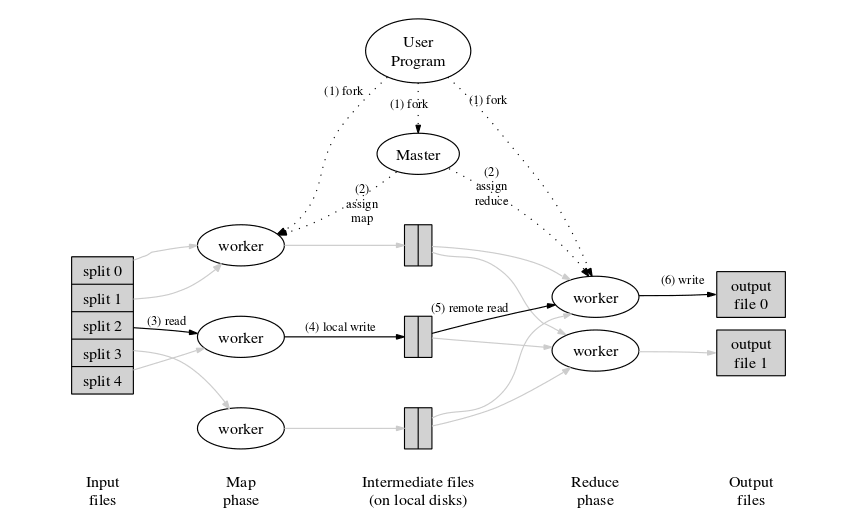
\includegraphics[width=\linewidth]{map-reduce-overview}
  \caption[MapReduce编程模型]{MapReduce编程模型(摘自Google MapReduce论文\cite{Dean2008})}
  \label{fig:map-reduce-overview}
\end{figure}

MapReduce由Google提出\upcite{Dean2008},最初被设计为用于分布式存储计算机集群,
部署在Google的服务器集群之上,执行大规模网络事务处理任务,如网页检索等,表现出很好的性能。
Apache基金会的Hadoop是分布式存储计算机集群上最著名的MapReduce实现。
L\"ammel使用Haskell语言给MapReduce的语义做了精确描述\upcite{Lammel2008}。

Ranger等\upcite{Ranger2007}在共享内存处理器上实现了MapReduce,名为Phoenix,
为MapReduce模型的处理过程提供了更多可配置选项。Phoenix-2是\upcite{Yoo2009}是Phoenix
的改进实现。

MapReduce也被移植到GPU上。香港科技大学的Bingsheng He等在Nvidia GPU上实现了
Mars\upcite{He2008},这是第一个运行在GPU上的Mapreduce系统。由于当时的GPU不支持
动态内存分配,Mars设计了一轮额外的\texttt{map\_count}阶段与一轮额外的\texttt{reduce\_count}
阶段,这带来了一定的附加开销。

MapCG\upcite{Hong2010}是MapReduce系统在GPU上另一版实现。MapCG的贡献是,
统一了MapReduce在CPU端与GPU端的接口设计,并在GPU上实现了一个轻量的动态内存分配器,
从而避免了Mars插入额外处理的开销。

Fang\upcite{Fang2011}增强了了Mars实现,使Mars可以运行在更多并行硬件之上,包括多核CPU、
Nvidia GPU、AMD GPU等,在开发CPU与GPU同时执行计算任务方面进行了一些尝试,
但并未取得理想效果。

Feng\upcite{Ji2011}与Chen\upcite{Chen2012}就GPU片上共享存储器的利用对MapReduce在GPU上
的实现分别提出了不同的优化措施。

Stuart设计了运行在GPU集群上的MapReduce系统GPMR\upcite{Stuart2011}。
出于性能考虑,GPMR向用户暴露了更多硬件细节。GPMR在\texttt{map}阶段
采用了了流水化的执行方式以重叠计算任务与设备间通信。

%% \section{GPU并行编程技术}\label{sec:gpu-parallel-prog}
%% 本节介绍当前使用最广泛的在GPU上进行通用编程的软件技术。

%% \subsection{CUDA}
%% CUDA架构是Nvidia公司针对自己的GPU提出的并行编程框架。
%% 它的提出对GPU通用编程技术产生了巨大的推动力。

%% CUDA为程序员提供了一个完整的GPU编程框架,将GPU的硬件结构
%% 清晰地展现出来。用户使用CUDA C编写在GPU上执行的程序,通常
%% 称为Kernel。CUDA C是一种对C语言的简单扩展,
%% 增加了若干关键字指定程序的执行位置(CPU还是GPU)、变量
%% 的存储位置(全局存储还是贡献存储),
%% 提供了一些内置变量一边获得某些运行时信息。

%% CUDA采用STMD编程模型,这是一种类似与SPMD的编程模型,
%% 一个Kernel程序被一组线程执行,执行路径一般和线程在组中所处的位置相关。
%% 线程按照层次化组织,grid

%% \subsection{OpenCL}

%% \subsection{OpenACC \& OpenHMPP}



%%% Local Variables:
%%% mode: latex
%%% TeX-master: "../main"
%%% End:

\begin{ack}
  衷心感谢导师 xxx 教授和 xxx 副教授对本人的精心指导。他们的言传身教将使我终生受益。

  感谢 \nudtpaper{},它的存在让我的论文写作轻松自在了许多,让我的论文格式规整漂亮了许多。

\end{ack}


\cleardoublepage
\phantomsection
\addcontentsline{toc}{chapter}{参考文献}
\bibliographystyle{bstutf8}
\bibliography{ref/refs}

\begin{resume}

  \section*{发表的学术论文} % 发表的和录用的合在一起

  \begin{enumerate}[{[}1{]}]
  \addtolength{\itemsep}{-.36\baselineskip}%缩小条目之间的间距,下面类似
  \item Yang Y, Ren T L, Zhang L T, et al. Miniature microphone with silicon-
    based ferroelectric thin films. Integrated Ferroelectrics, 2003,
    52:229-235. (SCI 收录, 检索号:758FZ.)
  \item 杨轶, 张宁欣, 任天令, 等. 硅基铁电微声学器件中薄膜残余应力的研究. 中国机
    械工程, 2005, 16(14):1289-1291. (EI 收录, 检索号:0534931 2907.)
  \item 杨轶, 张宁欣, 任天令, 等. 集成铁电器件中的关键工艺研究. 仪器仪表学报,
    2003, 24(S4):192-193. (EI 源刊.)
  \item Yang Y, Ren T L, Zhu Y P, et al. PMUTs for handwriting recognition. In
    press. (已被 Integrated Ferroelectrics 录用. SCI 源刊.)
  \item Wu X M, Yang Y, Cai J, et al. Measurements of ferroelectric MEMS
    microphones. Integrated Ferroelectrics, 2005, 69:417-429. (SCI 收录, 检索号
    :896KM.)
  \item 贾泽, 杨轶, 陈兢, 等. 用于压电和电容微麦克风的体硅腐蚀相关研究. 压电与声
    光, 2006, 28(1):117-119. (EI 收录, 检索号:06129773469.)
  \item 伍晓明, 杨轶, 张宁欣, 等. 基于MEMS技术的集成铁电硅微麦克风. 中国集成电路, 
    2003, 53:59-61.
  \end{enumerate}

  \section*{研究成果} % 有就写,没有就删除
  \begin{enumerate}[{[}1{]}]
  \addtolength{\itemsep}{-.36\baselineskip}%
  \item 任天令, 杨轶, 朱一平, 等. 硅基铁电微声学传感器畴极化区域控制和电极连接的
    方法: 中国, CN1602118A. (中国专利公开号.)
  \item Ren T L, Yang Y, Zhu Y P, et al. Piezoelectric micro acoustic sensor
    based on ferroelectric materials: USA, No.11/215, 102. (美国发明专利申请号.)
  \end{enumerate}
\end{resume}

% 最后,需要的话还要生成附录,全文随之结束。
\appendix
\backmatter
\chapter{Rat形式语法}\label{chap:formal-syntax}

\setlength{\grammarindent}{10em}
\setlength{\grammarparsep}{5pt}
\paragraph{Syntax Rules}
\begin{grammar}
<program>        ::=    <export>+ <top level unit>*

<export>         ::=    'export' <variable>

<top level unit> ::=    <type def>
                 \alt     <variable decl>
                 \alt     <variable def>

<type def>       ::=    'newtype' <type name> '=' <constructor> <type spec>

<constructor>    ::=    <variable>

<type spec>      ::=    <primitive type>
                 \alt     <struct type>
                 \alt     <vector type>
                 \alt     <type spec> '$\to$' <type spec>

<primitive type> ::=    'Int8' | 'UInt8' | 'Int16' | 'UInt16' \alt 'Int32' | 'UInt32' | 'Int64' | 'UInt64'
                 \alt     'Float' | 'Double'

<struct type>    ::=    '\{' <variable decl> (',' <variable decl>)* '\}'

<vector type>    ::=    '[' <type name> ']'

<variable decl>  ::=    <variable> '::' <type name>

<variable def>   ::=    <variable> <variable>* '=' <expression>

<expression>     ::=    <literal>
                 \alt     <variable ref>
                 \alt     <function app>
                 \alt     <lambda exp>
                 \alt     <vector comprehension>
                 \alt     <vector element ref>
                 \alt     <vector slice ref>
                 \alt     <conditional>
                 \alt     <let exp>
                 \alt     <where exp>
                 \alt     '(' <expression> ')'

<literal>        ::=    <number>
                 \alt     <boolean>
                 \alt     <character>
                 \alt     <tuple literal>
                 \alt     <vector literal>

<tuple literal>  ::=    '(' <literal> (',' <literal>)+ ')'

<vector literal> ::=    '[' <start> ',' <end> (',' <step>)? ']'

<start>          ::=    <number>

<end>            ::=    <number>

<step>           ::=    <number>

<variable ref>   ::=    <variable>

<function app>   ::=    <function ref> <expression>*

<function ref>   ::=    <variable>

<lambda exp>     ::=    '$\backslash$' <bind var>+ '$\to$' <expression>

<bind var>       ::=    <variable>

<conditional>    ::=    'if' <test> <if clause> <else clause>?

<test>           ::=    <expression>

<if clause>      ::=    <expression>

<else clause>    ::=    <expression>

<vector comprehension>
                 ::=    '[' <expression> \\('|' <generator> (',' (<generator> | <filter>))+ ']'

<generator>      ::=    <variable> '$\gets$' <variable>

<filter>         ::=    <expression>

<vector element ref>
                 ::=    <variable> '[' <index> ']'

<index>          ::=    <expression>

<vector slice ref>
                 ::=    <variable> '[' <index> ':' <index> (',' <index>)? ']'

<let exp>        ::=    'let' <variable decl>+ <variable def>+ 'in' <expression>

<where exp>      ::=    <expression> 'where' <variable decl>+ <variable def>+
\end{grammar}

\paragraph{Lexical Rules}
\begin{grammar}
<variable>       ::=    <lower id> | <special var>

<lower id>       ::=    <lowercase> (<alpha> | <digit> | '\_')*

<special var>    ::=    '+' | '-' | '*' | '/' | '\^'

<class name>     ::=    <upper id>

<type name>      ::=    <upper id>

<upper id>       ::=    <uppercase> (<alpha> | <digit> | '_')*

<alpha>          ::=    <lowercase> | <uppercase>

<lowercase>      ::=    'a' | 'b' | ... | 'z'

<uppercase>      ::=    'A' | 'B' | ... | 'Z'

<number>         ::=    <integer>
                 \alt     <floating>

<integer>        ::=    <decimal>
                 ::=    ('0O' | '0o') <octal>
                 ::=    ('0X' | '0x') <hexadecimal>

<decimal>        ::=    <digit>+

<octal>          ::=    <octit>+

<hexadecimal>    ::=    <hexit>+

<digit>          ::=    '0' | '1' | '2' | '3' | '5' | '6' | '7' | '8' | '9'

<octit>          ::=    '0' | '1' | '2' | '3' | '5' | '6' | '7'

<hexit>          ::=    <digit> | 'A' | 'B' | 'C' | 'D' | 'E' | 'F' | 'a' | 'b' | 'c' | 'd' | 'e' | 'f'

<floating>       ::=    <decimal> '.' <decimal> <exponent>?
                 \alt     <decimal> <exponent>

<exponent>       ::=    ('e' | 'E') ('+' | '-')? <decimal>

<boolean>        ::=    'true' | 'false'

<character>      ::=    ''' <ascii> '''

<whitespace>     ::=    <space> | <tab> | <newline> | <comment>

<comment>        ::=    '--' <any character>* <newline>
\end{grammar}


\end{document}
